\section{Solution}
Our description of our solution will be rooted in two major parts, as described in the introduction.
The following part regards our texture mapping and morphology.\newline

\subsection{Floor Tracking}
To get in touch with the concepts of morphology, our first assignment was to map the path of a person described by a video file. This mapping should be done, such that the path would correctly appear on an actual map.\newline

The videofile we were provided came accompanied by data related to the movement of the person.\newline

Solving this assignment required us to create the function \textsl{DisplayTrace(...)}, which processes the data and draws the trace onto the actual map. This function draws upon some properties of the \textsl{showFloorTrackingData()} function, and by its extension the \textsl{getHomographyFromMouse(...)} function.\newline

In the \textsl{DisplayTrace(img, points, H)} function we start out by going through all points provided by the list "points". These are created in the \textsl{showFloorTrackingData()} function, so we start our research there.\newline

The \textsl{showFloorTrackingData()} function finds the three boxes that contain the person which we are tasked to track. Each box determains a different part of the person; red is upper body, blue is complete body, and green is lower body. As such, we have chosen to track the "green box", which is the box that describes the feet of our target.
The feet should be the best point to go for, since it will be the most precise. Should the camera have a very sharp angle of attack, plotting from the face or torso could give very unaccurate results. The homography will be created such that the floor coordinates get malformed.\newline

\begin{figure}
	\centering
	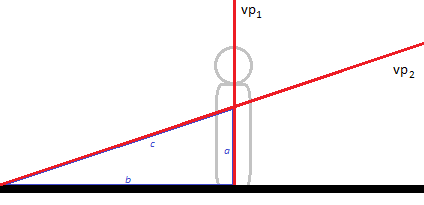
\includegraphics[scale=0.9]{images/viewpointdifference.png}
	\caption{Differences in viewpoints.}
	\label{fig:viewpoints}
\end{figure}

Looking at figure \ref{fig:viewpoints}, we can tell that the difference between the two points \(p1,p2\) on the base plane represented by \(vp_1\) is \(b_l\) when the angle of attack on \(vp_2\) is sharpened. The difference \(b_l\) is dependant on \(a_l\), given that \(b_l = \sqrt{c_l^2-a_l^2}\). \(c_l = \frac{a_l}{sin(A)}\)\newline

We have chosen the bottom middle spot of the green box, to avoid these complications. This should be the most precise point when considering its proximity to the ground, along with its position horizontally. Given the green box \(B_(x,y,w,h)\), we can find the best point \(p_(x,y)\) with the following calculations:
\[p_y = B_y+B_h \quad | \quad p_x = B_x + (B_w / 2)\]

Now that we have our point, we need to transfer it into a valid point on our map. We do this using a homography.

A homography has the interesting ability, that it is capable of turning one set of coordinates into another. This way, we can insert the coordinates of our traced pathing, and it will help us translate them to fit the map.

With the traced path in hand and translated, we can go paint the path onto the map, in our case, something that is done with the CV2 library and its \textsl{cv2.circle(...)} function.